\section{Tổng quan nghiên cứu}

Trong thời gian gần đây, nhiều nghiên cứu về hệ thống đa robot thao tác vật thể thông qua việc đẩy đã được thực hiện và công bố, tổng quan chi tiết có thể được tìm thấy trong \cite{tuci2018cooperative}. Với bài toán xây dựng cấu hình, các nhà khoa học trên thế giới đưa ra nhiều phương pháp tiếp cận khác nhau, tùy theo mục tiêu của từng phương pháp. Một trong những cách tiếp cận đơn giản nhất bao gồm xây dựng với một số lượng robot hoặc hình dạng vật cụ thể, ví dụ như là một hộp hình chữ nhật \cite{alkilabi2017cooperative}, cố định cấu hình robot theo một quy tắc nhất định như phân bố kín xung quanh vật thể, hoặc chia nhóm robot thành hai nhóm trái phải và điều khiển theo mô hình hai bánh vi sai \cite{nguyen2024distributed}. Các hướng này thường dễ tiếp cận, giúp giảm bớt tài nguyên tính toán để tập trung và chiến thuật điều khiển, tuy nhiên khá thiếu linh hoạt.  Một số hướng nghiên cứu thì lại coi việc tìm cấu hình như một bài toán tối ưu, và xây dựng những phương pháp đánh giá khác nhau các góc nhìn khác nhau về ổn định tiếp xúc, khả năng sinh lực-mô men, giới hạn ma sát hoặc hình học tương tác giữa robot-vật thể, và nhiều yếu tố khác. Một số hướng tiếp cận phổ biên bao gồm sắp xếp vị trí sao cho vật thể bị “giam” trong một miền hình học kín (caging) \cite{pereira2002decentralized}, chọn dựa trên các ràng buộc về hình học, ví dụ độ lợi về cánh tay đòn \cite{ebel2021nonprehensile}, chọn theo hướng lực muốn thao tác,\dots Các phương pháp dạng này thể hiện rõ ưu điểm về khả năng mở rộng cũng như tính linh hoạt của hệ đa robot, khi mà cho phép xử lý bài toán với số lượng robot và hình dạng vật thể bất kỳ, tuy nhiên yêu cầu tài nguyên tính toán cao, thậm chí cần xử lý tập trung. Nhìn chung mỗi hướng tiếp cận đều có những ưu và nhược điểm riêng, tùy thuộc vào cách tiếp cận mà sẽ có những phương pháp giải khác nhau để có thể tìm được các cấu hình này, sau đó tiếp tục tiếp tục xử lý bài toán tìm chiến thuật điều khiển tương ứng để đẩy vật.

Phần lớn các nghiên cứu về chiến thuật điều khiển đa robot phối hợp đẩy vật hiện này đều dựa vào điều khiển vị trí của robot (position based). Việc điều khiển theo vị trí là hợp lý, nhất là khi các robot di động thường được điều khiển trên tầng vị trí. Tuy nhiên, cách tiếp cận này cũng tồn tại nhiều hạn chế, chẳng hạn để đảm bảo vật thể có thể được vận chuyển thành công, một số lượng robot lớn thường phải được huy động vì không có cơ chế rõ ràng để xác định số robot cần thiết nhằm tạo ra lực đủ lớn, điều này có thể làm giảm tính bền vững của hệ thống. Hơn nữa, khi chỉ dựa trên thông tin vị trí, các robot cũng khó xác định chắc chắn liệu mình đã tiếp xúc với vật thể hay chưa, đặc biệt trong điều kiện nhiễu hoặc sai số hình học. Một điểm hạn chế nữa là robot không thể nhận biết được lực tác động lên vật thể và lên chính bản thân chúng, từ đó có nguy cơ gây ra lực tiếp xúc quá lớn làm hỏng robot hoặc vật thể. Về mặt điều khiển, khi chỉ sử dụng thông tin vị trí, vật thể bị xem như một nhiễu tác động lên bộ điều khiển vị trí của robot thay vì là mục tiêu thao tác cần đạt được. Những hạn chế này cho thấy tầm quan trọng của các phương pháp dựa trên điều khiển lực, khi mà nó cho phép đo đạc và kiểm soát trực tiếp các lực tương tác giữa robot và vật thể, từ đó thậm chí có thể hướng tới việc lựa chọn đội hình dựa trên đặc tính động lực học. Dù chưa phổ biến bằng các phương pháp điều khiển vị trí, một số nghiên cứu gần đây đã cho thấy triển vọng đáng kể của hướng tiếp cận dựa trên điều khiển lực đối với bài toán vận chuyển vật thể không cầm nắm bằng nhiều robot. Trong \cite{wang2016kinematic,wang2015multi} các robot trong bầy sẽ cảm nhận và khuếch đại lực được tạo ra bởi một robot chỉ huy (leader) để di chuyển một hộp hình chữ nhật, hay trong \cite{neumann2014object,neumann2016hybrid} một bộ xử lý trung tâm ở ngoài sẽ tính toán ra lực mong muốn rồi truyền cho hai robot để đẩy vật theo một đường thẳng. Tuy là một hướng tiếp cận khá mới và khó, nhưng điều khiển dựa trên lực đã thể hiện được các ưu điểm nổi bật so với phương pháp theo vị trí, đây cũng là hướng mà đồ án này được xây dựng theo.

Các yếu tố về đến mặt hình học của thể cần thao tác đóng vai trò quan trọng đối với việc xây dựng và điều khiển đội hình trong lĩnh vực thao tác vật thể nói chung và đẩy vật nói riêng. Trong các nghiên cứu ở trên, đa phần các tác giả sẽ giả định là có trước các thông tin này. Tuy nhiên trong thực tế, khác với đặc trưng về hình dạng vật thể vốn có thể đo lường dễ dàng bằng các phương pháp như camera từ trên xuống (top-down camera), quét bằng lidar lúc mapping, hoặc sử dụng cảm biến xúc giác (tactile sensor), thì vị trí điểm trọng tâm (COM - Centre of Mass) thường rất khó để xác định nếu như nó không trùng với tâm hình học của vật thể. Lúc này cần phải xử lý một bài toán mới đó là ước lượng vị trị khối tâm của vật dựa vào tương tác đẩy trước khi tiến đến tìm đội hình và lên chiến lược đẩy vật. Dựa trên tính chất cơ bản của COM là khi vector lực đẩy tác dụng đi qua điểm này sẽ không sinh ra mô men xoay, và ngược lại nếu không đi qua thì sẽ sinh ra mô men dẫn đến chuyển động xoay của vật, rất nhiều phương pháp khác nhau đã được để ra để ước lượng vị trí tương đối của COM. Các nghiên cứu tập trung hoàn toàn vào việc xác định trọng tâm hiện nay phần lớn sử dụng robot tay máy và phương pháp học từ dữ liệu (data-driven) như \cite{bauza2019estimating} mang lại kết quả khá tốt, điều này lại khó áp dụng được trong hệ đa robot di động chỉ có cơ cấu đẩy do yêu cầu lực cần thiết để đẩy vật và lượng dữ liệu lớn cần thu thập trong thời gian dài. Một số nghiên cứu sử dụng robot động đã đề xuất các phương pháp ước lượng đơn giản thông qua việc đẩy thử và theo dõi chuyển đông quay của vật, sau đó thu hẹp phạm vi mà vùng điểm trọng tâm có thể nằm trong đó bằng phương pháp chặt nhị phân \cite{jeong2020zeromoment,chitta2010onboard}. Tuy kết quả mang lại tương đối khả quan, các phương pháp này lại bộc lộ rõ yếu điểm khi yêu cầu phải đẩy qua được điểm trọng tâm để kết thúc tìm kiếm, điều mà không phải lúc nào cũng có thể đạt được nếu chỉ đẩy vuông góc với cạnh của vật ví dụ như vật hình ngôi sao, hay yêu cầu sinh những lực khác với lực pháp tuyến. Ngoài ra thì tùy vào độ phân giải mà số lượng lần đẩy của các phương pháp này có thể tương đối lớn, do mỗi lần ta chỉ chia đôi được không gian tìm kiếm khi điều kiện dừng là phải đẩy qua được COM. Đồ án này sẽ đề xuất một phương pháp hỗ trợ xác định trọng tâm thông qua cơ chế đẩy bằng robot di động yêu cầu số lần đẩy thử thấp dựa trên một yếu tố thường không ứng dụng được với robot tay máy là gia tốc góc.

\begin{figure}[h]
    \centering
    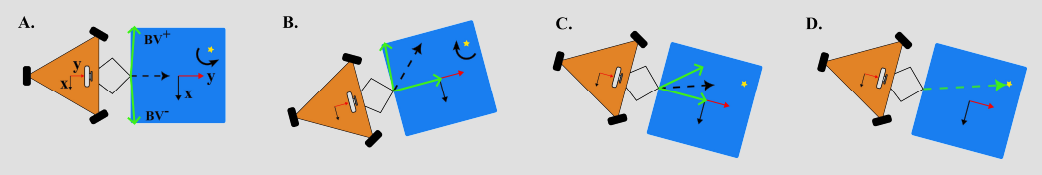
\includegraphics[width=1\textwidth]{chapter1/image/cnp.png}
    \caption[Robot đẩy thử để xác định điểm trọng tâm bằng phương pháp chặt nhị phân]{Hình 1 từ \cite{chitta2010onboard}: Robot đẩy thử để xác định điểm trọng tâm bằng phương pháp chặt nhị phân }
    \label{fig:cnp}
\end{figure}
